% Johnathan Fritsche

The CD4007 gate array was used to make a two-input NOR gate.


\FloatBarrier

\begin{figure}[h!]
\centering
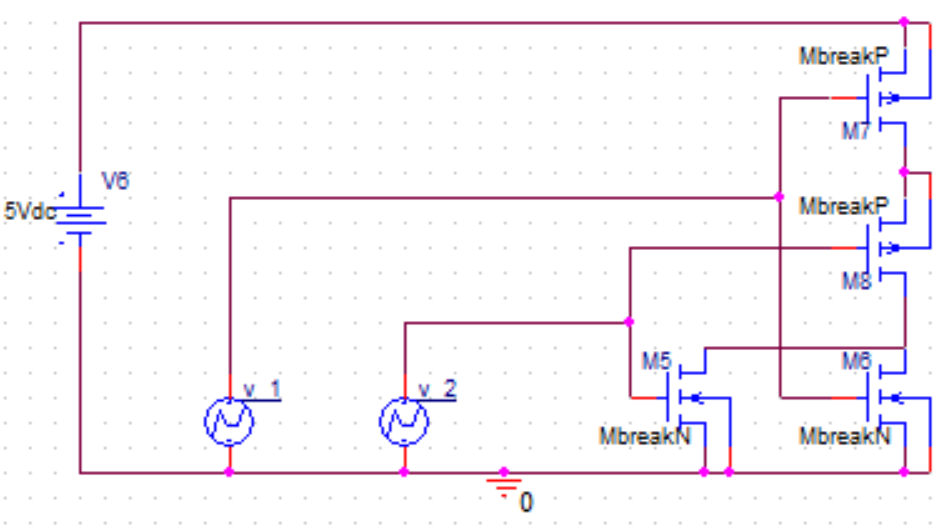
\includegraphics[scale=0.5]{../images/nor_schematic.PNG}
\caption{The two-input NOR gate circuit.}
\label{fig:nor_schematic}
\end{figure}

\FloatBarrier

The two-input NOR gate operates such that the output will be high only when both inputs are low. Otherwise, the output will be low. It can be shown from the circuit above that $V_1$ and $V_2$ serve as the inputs and $V_{out}$ is taken across the drain of $M8$ to the ground.


\FloatBarrier

\begin{table}[h!]
\centering
\csvautotabular{../data/logic_nor.csv}
\caption{Logic of the two-input NOR gate.}
\label{tab:logic_nor.csv}
\end{table}

\FloatBarrier

The analysis of this circuit shows that the behavior of the two-input NOR gate is consistent with our logic table and our expectations. The figure below shows the results of the NOR gate simulation.

\FloatBarrier

\begin{figure}[h!]
\centering
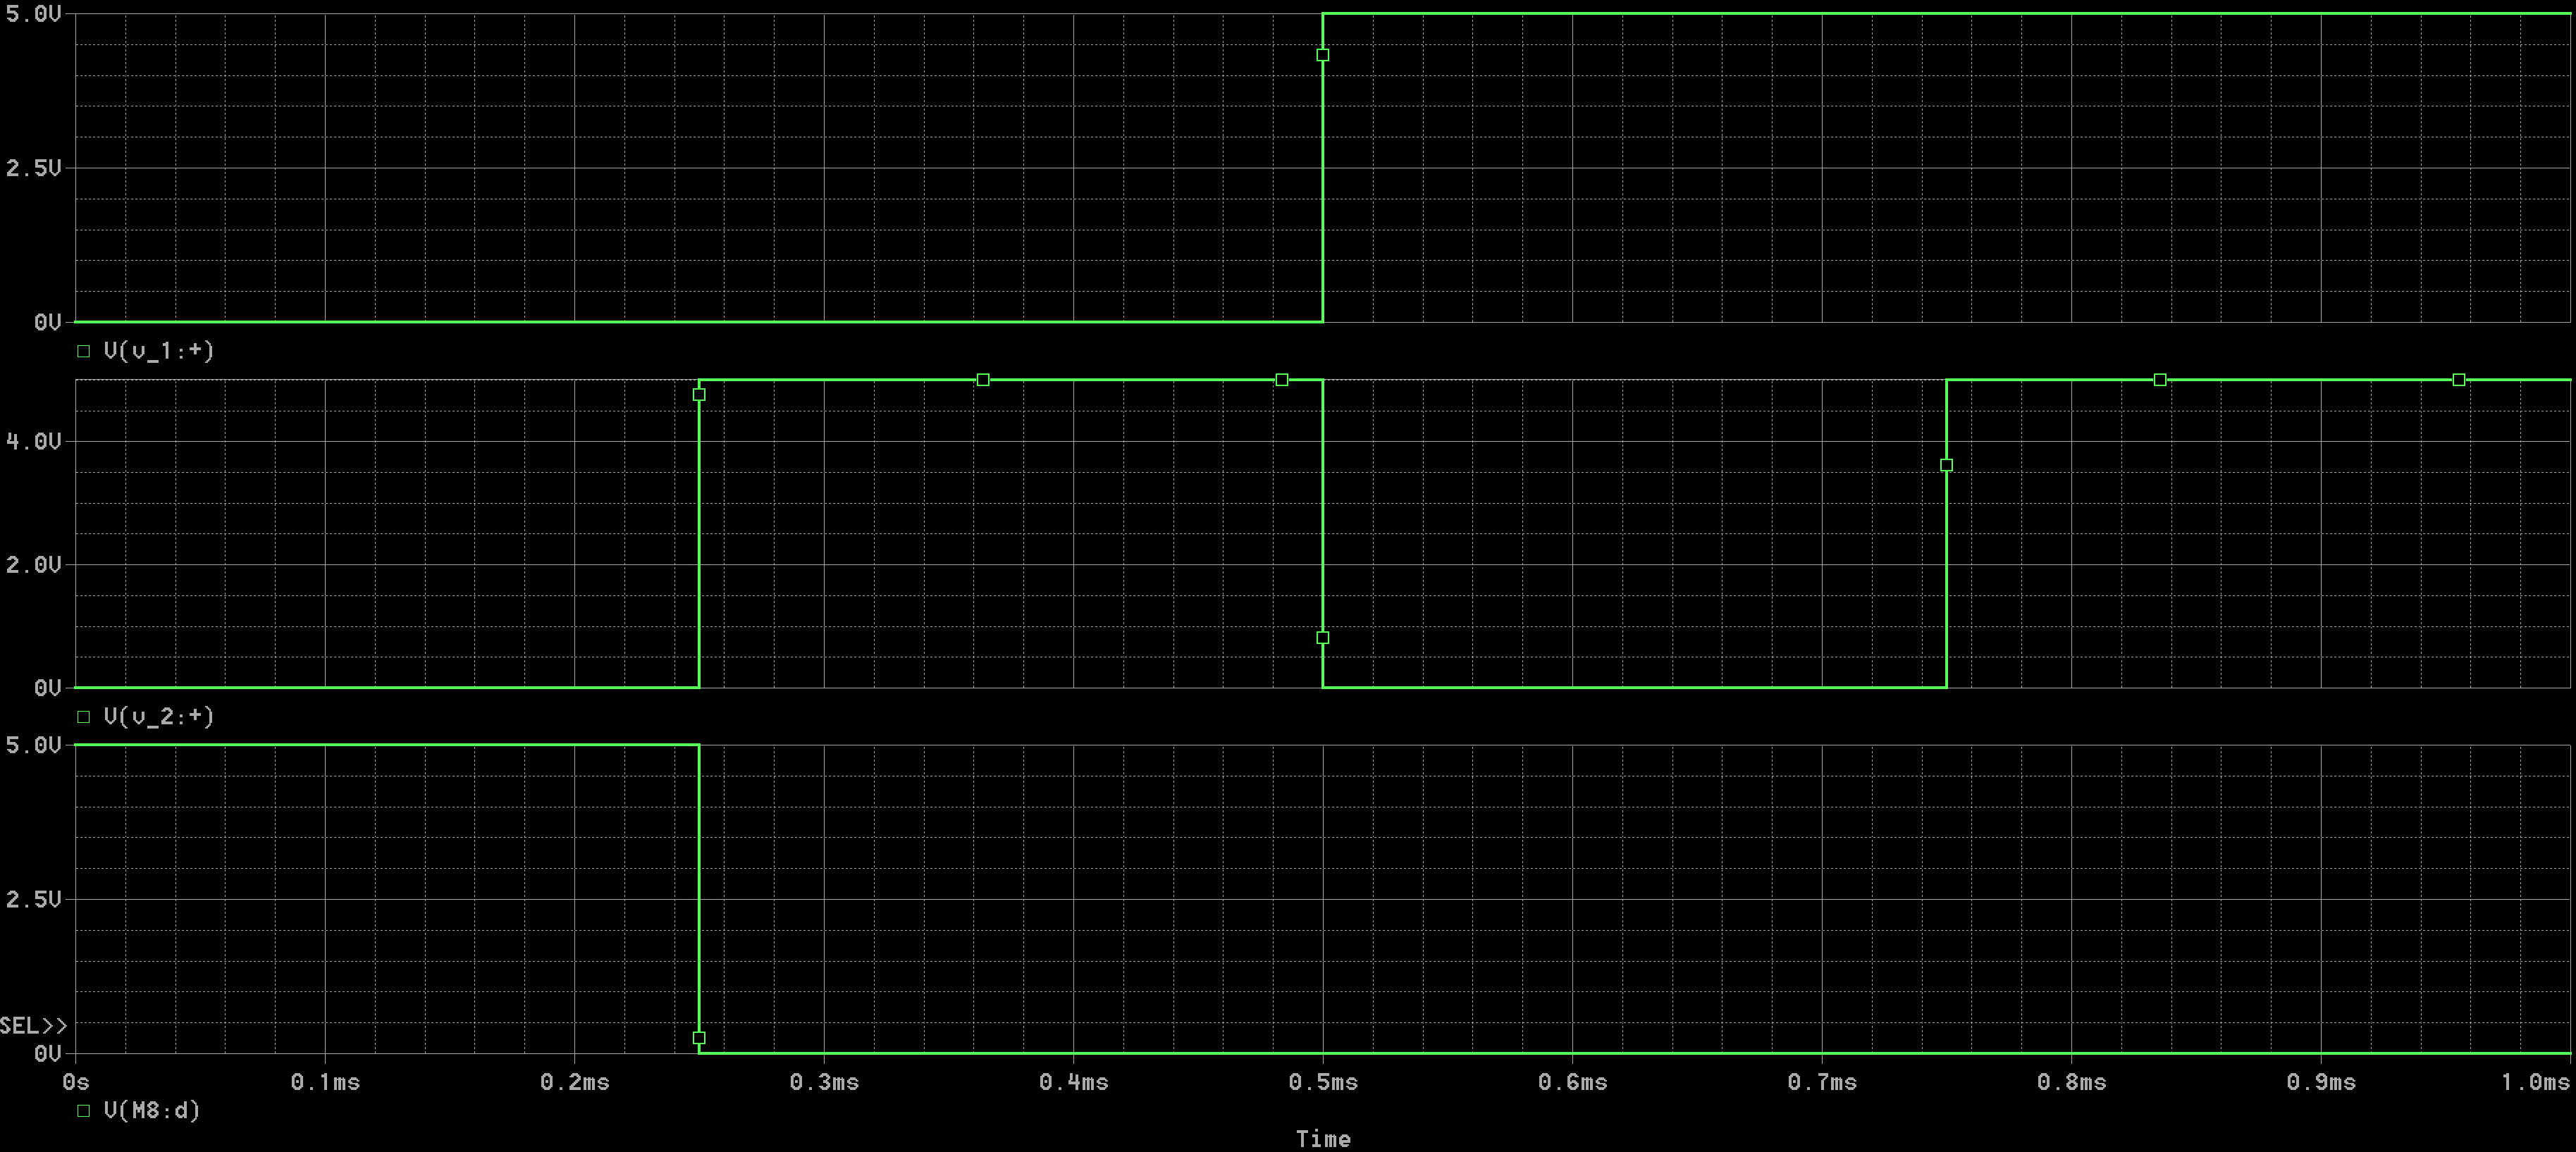
\includegraphics[scale=0.3]{../images/nor_transient_output.PNG}
\caption{Simulation output of the NOR gate.}
\label{fig:nor_transient_output}
\end{figure}

\FloatBarrier

Using $V_1$ and $V_2$ as the inputs, we see that the output, $M8$, of our NOR gate will only be high when both inputs are low. This proves that our expectations for the NOR logic and circuit structure are correct; however, this is still a simulation. Due to some complications with the CD4007 and breadboard, the results are only available from a SPICE simulation.
